\chapter{Implementation}
\label{IMPL}
This chapter describes how we have implemented some of the more interesting
features of the software. We aim to describe it to enough detail that this
chapter can serve as a guideline for implementing the functionalities we
describe.
\section{UTM-conversion}
\label{IMPL-UTM}
When the graphical user interface part of the map tries to communicate with the
model through control, some conversions of the different kind of values are
necessary. Both when going from coordinates in the java-coordinate system to
UTM32-coordinates and back. 

We need to convert the values when we want to use the mousezoom and when we want
to place the markers for pathfinding. We get an input on the graphical user
interface when we mousezoom and this needs to be converted to UTM-coordinates so
that we can create the new boundaries of the zoomed rectangle.

When we place markers for pathfinding, we do the same as when we do mousezoom,
but instead we store the point as UTM32-coordinates and whenever we move the
map, we convert it back to pixel-coordinates so that we know where to draw.

The java-coordinates have origo in the top left corner with the y-coordinate
increasing the further down the y-axis you go. UTM32-coordinates are a bit
different. UTM32 has origo in the bottom left corner and the y-coordinate
increasing the further up you go on the y-axis.

We have a utility class with methods for converting the points back and forth.
One takes a point from the view, the model and the view itself uses this formula
for converting the pixelpoint to the UTM32-point.




a$_y$ = canvas$_{height}$ - a$_y$

UTM$_x$ = bounds$_x$ + (a$_x$ / canvas$_{width}$) * bounds$_{width}$

UTM$_y$ = bounds$_y$ + (a$_y$ / canvas$_{height}$) * bounds$_{height}$

return \class{point}(UTM$_x$, UTM$_y$)

Below is an illustration of the conversion from pixel to UTM.

\begin{figure}[!ht]
\centering
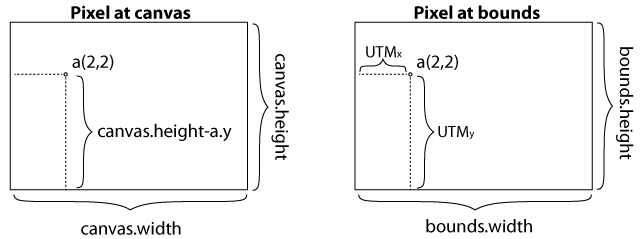
\includegraphics[width=0.5\linewidth]{images/UTMillu}
\caption{UTMillustration}
\label{fig:UTMconversion}
\end{figure}

To convert from UTM to pixels we use the same formula but reversed.

Pixel$_x$ = ((a$_x$ - bounds$_x$) / bounds$_{width}$) * canvas$_{width}$

Pixel$_y$ = ((a$_y$ - bounds$_y$) / bounds$_{height}$) * canvas$_{height}$

Pixel$_y$ = canvas$_{height}$ - Pixel$_y$

return \class{point}(PIXEL$_x$, PIXEL$_y$)

\section{Mousezoom}
\label{IMPL-MZ}
We have implemented the mouse zoom requirement by using \class{mouseEvent}s on
our canvas. When the user presses the left mouse button down, it generates a
\class{mousePressed} event. We record the position of the mouse at the time of
the \class{mousePressed} event and wait for the \class{mouseReleased} event.
When the left mouse button is released, it generates a \class{mouseReleased}
event. We use the position of the mouse at the \class{mouseReleased} event and
the \class{mousePressed} to calculate new bounds for the model.



As mentioned in section \ref{IMPL-UTM} \class{\nameref{IMPL-UTM}}, we use
UTM-conversion to convert pixel values into the UTM values we need.

Often the user will not drag a square that is in perfect ratio with the
canvas. If it does not have the same ratio as the canvas, we change the ratio
of the dragged square behind the scenes. We do this by either adding length or
width to the dragged square. We always make sure to at least show what was
inside the box the user dragged.

If the ratio of the dragged square is smaller than the canvas ratio, we make the
dragged box wider. If the ratio of the dragged square is larger, we make the
dragged box taller.

\section{Dijkstra vs A-star}
\label{IMPL-DVA}
In preparations to implementing the path finding feature to our program, we knew 
two possible choices. They are named Dijkstra and A* (A-star), and are quite 
similar but behave a little different.

The Dijkstra algorithm uses a minimum priority queue to find the shortest path 
from a given node to every other node by looking at the edges connecting nodes. 
The program will take a node from the priority queue and add all the other nodes 
that are connected from the current to the priority queue. The priority queue 
takes a value to the node and this should be the distance to the current node 
plus the length of the edge between the two. Since the priority is made to return 
the node with the smallest value associated with it, the next node in line will 
always be the one which is closest to the start node. This procedure continues 
until all nodes have been visited and by logging what edge led to all the nodes 
it is possible to trace back the route to the start node.

This algorithm is great if need to find the distance from one point to many other 
points, but can be quite slow since it just searches in all directions without 
concerns to the direction of the target node.

This is where A* comes in handy. The A* algorithm is a modification to Dijkstra 
that also looks at the estimated distance from the given node when determining 
the value for the priority queue. When using the geographical distance as a 
measure of best route the value would be the current distance from the start 
node plus the direct distance to the target (as if there were a road directly to 
the target). With this subtle change the algorithm will prioritize nodes that are 
relatively closer to the target rather than those that are in the other
direction. This makes the algorithm much faster since it will not pay much attention to the roads 
that are not in the direction of the target.
We have decided to use the A* algorithm since we only calculate routes between 
two distinct nodes and therefore don`t need the route from the start node to all 
others. The time reduction that A* gives is also a definite plus since no user 
wants to sit and wait too long for the program to find the route.

%M�ske vi skulle have pointen med om hvilket transportmiddel A*star virker bedst
% med?

\section{Evaluator}
\label{IMPL-EVA}
In order to make our path finding algorithm flexible enough for different 
interpretations of the ``best route'', we have added an entity called \class{Evaluator}. 
This is an object that has the responsibility of evaluating a node relative to 
the target node. The \class{Evaluator} also has the responsibility of calculating the 
heuristics that the A* algorithm relies on. By using the \class{Evaluator} we are able to 
use the same path finding algorithm for two very different tasks, namely the 
biking route and the car route. The major difference between these is that the 
bike uses the distance and the car uses the total drive time. This implementation 
is also a good example of making our code ready for future features, since if we 
needed to add other means of transportation or simply variations of the ones we 
have, we would only need to create new \class{Evaluator} objects and not change a single 
line of code in the A* algorithm.

\section{Quadtree}
\label{IMPL-QT}
In order to improve the drawing of our map, we have implemented the data
structure Quadtree. The Quadtree divide our road data into smaller rectangles.
When we want to retrieve data from the map, we can give the quadtree a
rectangle, and it will return all the roads within rectangles that intersect
that rectangle. This technique optimizes the drawing of the roads, because we
don�t draw roads outside of the view. However, when viewing the entire map of
Denmark, this implementation does not help us. Therefore, it is necessary to
only to draw the bigger roads when zoomed out. We have discussed two different
techniques to do this. The first technique relayed on putting the bigger roads
at the top of the quadtree when building it. Then we could specify at which
depth we wanted to search the quadtree. The second technique relayed on dividing
the quadtree into different parts, each containing their own road types. Going
with this implementation, we simply specify which roads we want to draw. This
method requires more RAM than the first one, because it requires more instances
of object QuadTreeNode.
%MAKE ILLUSTRATIONS
At first glance, the first method seemed to be superior to the second, because
it saves some RAM. However, the second implementation is easier to implement,
and the extra RAM are such a small percentage of the overall RAM use, that it
does not really matter.

\section{Serialization}
\label{IMPL-SERI}
We observed that the user had to wait quite a long time for the program to start. This 
was because every time we start the program, we loop through the entire dataset given 
to us by Krak. This data-set is huge, and because of this it takes quite a lot of time to 
start the program. Because we need to load all these data, the user is presented with 
a blank screen for a long time, before all these data are loaded and the program starts.

We started looking for a way to speed up the loading process, so the user has a map in 
front of him or her quickly, when the user starts the program. What takes the most time 
is looping through the data and creating the needed datastructures (quadtrees, the 
graph and so on), so if we could skip these steps or speed them up, we could save a lot 
of time.

This is where serialization comes into play. By serializing an object, you transform your 
object into something that can be passed around, through streams and such. So by 
serializing objects, you can save them to files. If the object to be serialized contains 
references to other objects, these will also be serialized (if they are Serializable / 
implements java.io.Serializable).

By doing this, we only need to build our datastructures the first time you start the program. 
After the objects have been created, they are been serialized and saved to files. The next 
time the user starts the program, we check whether the data has been changed. We check 
this by checking the MD5 checksum of the file, with \class{MD5Checksum} (we didn't write 
this class ourselves). When we serialize the objects, we also save the checksum to a config 
file. If the data hasn't been changed (i.e. the checksum is the same), we load the objects that 
we saved, instead of making them all over.

We serialize all the quadtrees, the graph and the maxbounds-object (specifying the bounds 
of Denmark), as these are the objects we need for the program to run. When saved to the 
harddrive, it is around 65MiB, which is okay, given the sizes of harddrives today.

We save all these objects to one single file, in order to keep the references. If we didn't do 
this, the references will be ruined, which can break the program. We experienced problems 
with this, as nodes and edges is both stored in the quadtrees and the graph. If we serialized 
and saved the quadtrees in one file, and the graph in other file, a given node will be saved 
twice, and when we load the data from the serialized files, the node will exist twice, and it 
won't be the same node. But if we save the objects to a file through the same stream, we only 
get one of each, which leads to less RAM usage, less harddrive usage, faster loadtimes and 
fewer bugs.

\subsubsection{Threading}
By serializing our main objects, we cut several seconds of our load times. But we can do it 
even faster. We are serializing several objects, but only few of them are needed right from 
the start of the program. So what we can do to speed it up even more, is loading the few 
necessary objects, and then load the rest in the background. We do this with threads. 
We load the few objects we need from the start, then create a new thread to load the rest 
of the objects, and in the mean time, we create the window and draw the map.

The same goes for the first run. The user doesn't need to wait for the program to finish 
serializing and saving to files. By using threads, we can create the datastructures, and 
then immediately show the window to the user, while saving the objects to files in the 
background.
